 \documentclass{article}
\usepackage[francais]{babel}
\def\printlandscape{\special{landscape}}    
\usepackage{amsmath}
\usepackage[utf8]{inputenc}
\usepackage[T1]{fontenc} 
\usepackage{fancybox} 
\usepackage{alltt}
\usepackage{graphicx}
\usepackage{lmodern}
\usepackage[colorlinks,hyperindex,bookmarks,linkcolor=blue,citecolor=blue,urlcolor=blue]{hyperref}
\usepackage{epsf}
\usepackage{enumitem}
\usepackage{pifont}
\usepackage{hyperref}
\usepackage{authblk}
\usepackage{titling}
\usepackage{floatflt}

\renewcommand{\maketitlehooka}{
 \begin{center}

\includegraphics[width=5cm, keepaspectratio=true, height=5cm]{Logo_Polytech_Sorbonne-2.png}\hfill
\includegraphics[width=5cm, keepaspectratio=true, height=5cm]{Logo_Sorbonne_Universite-2.png}
\end{center}
   
\centering
\vspace{1cm}
\title{\vspace{\fill}\textbf{ Rapport de projet pluridisciplinaire :} \newline Diffusion non linéaire en sciences de la terre modélisation des glaciers\vspace{\fill}}


\begin{center}
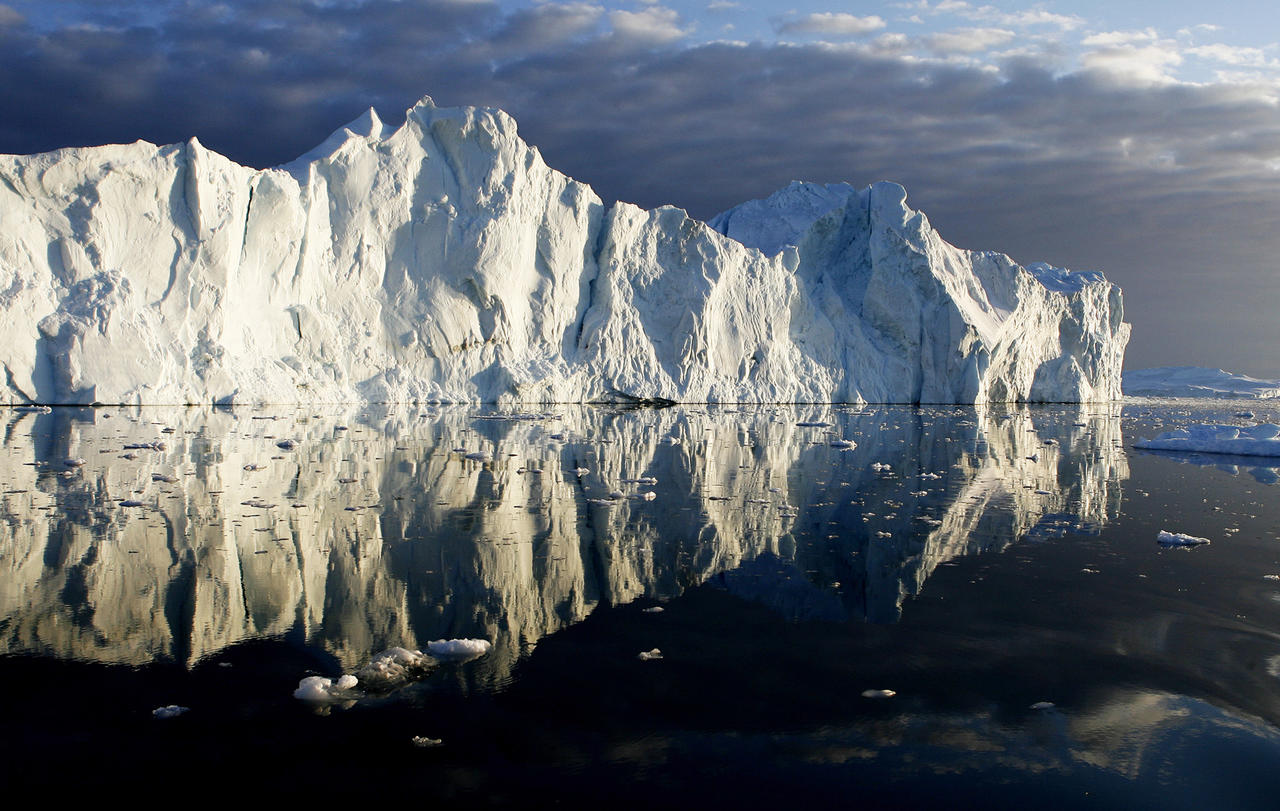
\includegraphics[width=9cm, keepaspectratio=true, height=8cm]{rtr1qbn7}    
\end{center}
    }


\author{Tania Mendes, Mathieu Nguyen, Samson Petros,\\ Yazid Bouhria, Elyas Assili, Maryam Aarab}

\affil{\textbf{Encadrante} : Laetitia Le Pourhiet}
\begin{document}
\maketitle 

\newpage

\tableofcontents

%-----------------------------------------------------------
\newpage
%\section{Introduction}\label{sec:intro}
\section*{Introduction}
\addcontentsline{toc}{section}{Introduction}

L’écoulement d’un glacier dépend de plusieurs facteurs qui sont principalement l’accumulation de neige, la fonte de glace, la gravité et le niveau de la pente du lit rocheux.
Les écoulements sont considérés incompressibles, visqueux et non linéaires, d’où l’intérêt de les modéliser avec les relations de Stokes.
\newline
C'est un processus continu, mais il est très difficile de les résoudre analytiquement. Pour cela, les modélisateurs utilisent donc des méthodes numériques.
L’intérêt ici va être d’énoncer les \textbf{relations générales de Stokes} appliquées aux glaciers, d’énoncer le modèle \textbf{Shallow Ice Approximation (SIA)} afin d’en déterminer les avantages et les limites dans l’analyse de l’écoulement d’un glacier en fonction du temps.


Dans le cadre de ce projet, nous allons utilisé le langage \textbf{Julia} pour la résolution de systèmes d'équations différentielles par \textbf{différences finies} afin de pouvoir prédire l'écoulement glaciaire du Groenland. \\ Nous utilisons Julia car c'est un langage de programmation moderne, polyvalent et qui permet de parralèliser des GPU sans demander trop de ressources. C'est un langage créé en 2009 par des chercheurs et ouvert au grand public en 2012. C'est un langage de haut niveau, dynamique et conçu pour des calculs scientifiques. Sa syntaxe est similaire à Python, R ou encore Matlab.


%-----------------------------------------------------------
\section{Présentation des méthodes de résolution}

\subsection{Les équations de Stokes}

Les équations de Stokes \cite{site1} ont comme principal objectif de décrire les \textbf{mouvements des fluides}. 
Pour procéder correctement, il faut connaître sa vitesse en tout point de l'espace : son champ de vitesse. Ainsi les équations de Stokes permettent de décrire le \textbf{champ de vitesse} d'un fluide. 

Afin de pouvoir appliquer ces équations dans le cas des écoulements des glaciers, nous considérerons ces derniers comme des fluides \textbf{incompressibles}, \textbf{visqueux} et \textbf{non linéaires}. Il s'agit d'un système d'équations pouvant être appliqué à tout type de glacier.

Ce système permet une très grande précision dans les résultats puisqu'il prend en compte toutes les contraintes au nombre de neuf, qu’elles soient longitudinales, transversales, verticales ou encore horizontales. 


Les équations de stokes peuvent être assimilé à la \textbf{seconde loi de Newton} appliquée aux fluides,
\begin{equation}
\sum\vec{F}=m\vec{a}
\end{equation}
, avec  $\vec{F}$ les forces s'exerçant sur le volume en $kg.m.s^{-2}$ ou $N$, $m$ sa masse en $kg$ et  $a$ son accélération en $m.s^{-2}$.
\newpage
Le nombre de Reynolds $Re$, qui représente le rapport entre les forces d'inertie et les forces visqueuses,
 \begin{equation}
\textit{Re} = \frac{\rho V L}{\mu}
\end{equation}
avec $\rho$ la masse volumique en $kg.m^{-3}$, $V$ la vitesse caractéristique en $m.s^{-1}$, L la dimension caractéristique en $m$ et $\mu$ le coefficient de viscosité en $m^{2}.s^{-1}$, caractérise les différents types d'écoulements. \\
Dans le cas des glaciers, le nombre de Reynolds est considéré comme petit car les glaciers sont égalés à des fluides très visqueux et pas conséquent le coefficient de viscosité $\mu$ est très élevé. On en déduit que les écoulements se font très lentement et donc nous pouvons \textbf{négliger le deuxième terme de la seconde loi de Newton} :
\begin{equation}
\sum\vec{F}= 0
\label{somme force}
\end{equation}


%%Les termes qui vont suivre sont explicités dans le cours "Introduction à la dynamique des fluides visqueux" de Thierry Menand.\cite{menand2020introduction}
La somme des forces est ainsi la somme des forces de volume $\vec{F}v$ induites par la gravité et qui agissent sur tout le volume, et des forces de surface $\vec{F}s$ qui sont induites par les frottements sur les bords et à l'intérieur de la glace.
\\\\
\begin{enumerate}
\item \textbf{Forces de volume}\\
Les forces de volume  $\vec{F}v$ induites par la gravité, et donc le poids, agissent sur toutes les particules d'un volume élémentaire et s'écrient :
\begin{equation}
\vec{F}v = \Delta_{m} \vec{g}
\end{equation}
avec $\Delta_{m}$ la masse élémentaire en $kg$ et $g$ l'accélération de la pesanteur en $m.s^{-2}$.
La masse élémentaire $\Delta_{m}$ peut se réécrire,  
\begin{equation}
\Delta_{m} = \int \rho dV = \rho dxdydz
\end{equation}
, avec $\rho$ la masse volumique en $kg.m^{-3}$, $dV=dxdydz$ le volume élémentaire de côtés $dx$, $dy$ et $dz$, en $m^{3}$.

Ainsi la $\vec{F}v$ la force de volume est : 
\begin{equation}
\vec{F}v = \int \rho \vec{g} dV
\end{equation}

\item \textbf{Forces de surface}\\
\end{enumerate}
Les forces de surface $\vec{F}s$ sont les frottement au bord et à l'intérieur du glacier. Pour le cas d'un glacier nous prenons en compte les contraintes normales à la surface $\sigma$ : 

\begin{equation}
\vec{F}s = \int \sigma \vec{n} dS 
\end{equation}
avec $\vec{n}$ le vecteur normal à la surface dirigé vers l'extérieur et $\sigma$ le tenseur de contrainte.\\
Le théorème de divergence permet de réécrire $\vec{F}s$ :
\begin{equation}
\vec{F}s = \int \nabla \sigma dV 
\label{force surface}
\end{equation}

Le tenseur de contrainte $\sigma$,
\begin{equation}
\sigma = 2 \mu \dot \varepsilon - I_{d}P
\end{equation}
avec $\mu$ le coefficient de viscosité en $m^{2}.s^{-1}$, $\dot \varepsilon = \frac{1}{2}( \nabla v + \nabla v^t\ ) $ le taux de déformation , $I_{d}$ la matrice identité et $P$ la pression en $Pa$ ou $kg.m^{-1}.s^{-2}$ .   \\ 
$2\mu \dot \varepsilon$ est la partie qui concerne la déformation et $I_{d}P$ est la partie isotrope. Le taux de déformation $\dot \varepsilon$ est un paramètre capital en rhéologie qui est l'étude de la déformation des écoulements sous l'effet des différentes contraintes appliquées.
\\\\
En intégrant l'expression du tenseur de contrainte dans ~\eqref{force surface} on obtient :
\begin{equation}
\vec{F}s = \int \nabla(2 \mu \dot \varepsilon - I_{d}P ) dV =  \int \nabla 2 \mu \dot \varepsilon dV - \int \nabla P dV
\end{equation}


Ainsi en récapitulant la somme des forces ~\eqref{somme force},
\begin{equation}
\begin{split}
\sum\vec{F} = \vec{F}s + \vec{F}v = 0 \\
\Leftrightarrow 
\int \nabla 2 \mu \dot \varepsilon dV - \nabla \int P dV + \int \rho \vec{g} dV = 0 \\
\Leftrightarrow 
- \int \nabla 2 \mu \dot \varepsilon dV + \nabla \int P dV = \int \rho \vec{g} dV  \\
\Leftrightarrow 
- \nabla 2 \mu \dot \varepsilon + \nabla P = \rho \vec{g}
\end{split}
\end{equation}


Ainsi, nous retrouvons bien l'expression des équations de stokes 
\begin{equation}
\left\{
\begin{array}{l}
-div(2 \mu \dot \varepsilon(\vec{v})) + \nabla P = \rho \vec{g} \\
div(\vec{v}) = 0 \qquad
\end{array}
\right.
\label{eq1}
\end{equation}
avec $\nabla = ( \frac{\partial}{\partial x} + \frac{\partial}{\partial y} + \frac{\partial}{\partial z})$, $v$ la vitesse en $m.s^{-1}$, $g$ l'accélération de pesanteur $en m.s^{-2}$, $\rho$ la masse volumique en $kg.m^{-3}$, $\mu$ le coefficient de viscosité $m^{2}.s^{-1}$ et $\dot \varepsilon$ le taux de déformation. Les écoulements sont incompressibles donc il n'y a pas de variation de volume ce qui se traduit par $div(\vec{v}) = 0$.
\newpage
Néanmoins, le \textbf{Groenland} est une calotte grande de milliers de kilomètres. Il faut alors un nombre considérable de points pour résoudre ces équations. De plus du fait de la complexité de celles-ci ainsi que des géométries de la calotte, cela est \textbf{coûteux en temps de calcul}. 
\\\\
Il existe de nombreuses simplifications de ces équations afin de minimiser le temps de calcul. Parmi elle, une des plus connue est l'approximation de la couche mince (\textbf{Shallow Ice Approximation}) appliquée pour la première fois sur la glace par Kolumban Hutter (1983). Ce modèle permet de réduire le problème de résolution 3D à un \textbf{problème 2D}. Il permet des calculs beaucoup plus simples. Ainsi, les calottes étant relativement minces, soit quelques kilomètres d'épaisseur, nous pouvons négliger les variations verticales de la vitesse les contraintes de cisaillement longitudinales et utiliser le modèle de l'approximation de la couche mince.
\newline

\subsection{Shallow ice approximation (SIA)}


Pour cette partie, nous nous sommes renseignées à travers le cours de Martina Schäfer \cite{schafer2007modelisation} et aussi grâce à un article publié dans le Cambridge University Press  \cite{seroussi_morlighem_rignot_khazendar_larour_mouginot_2013}.
\newline
D'après une étude de Robin Chatelin \cite{site3}, des chercheurs assurent que la résolution du système des équations de Stokes est \textbf{très coûteuse en temps} pour des applications réalistes (avec une complexité de \textbf{nlog(n)}). C'est pour cette raison qu'ils utilisent une simplification de ces équations basée sur le fait que, sur de très grandes calottes, l'\textbf{épaisseur est extrêmement faible} par rapport à la dimension horizontale. Pour cela, nous allons utiliser le modèle SIA (Shallow Ice Approximation). Sa validité dépend du \textbf{rapport d'aspect caractéristique $\zeta$} des objets glaciaires :
\begin{equation}
\zeta = \frac{e}{L}
\label{eq2} 
\end{equation}

Avec e l'épaisseur du glacier en $m$ et L la largeur du glacier en $m$. \\
Ce rapport est par exemple de $10^{-3}$ pour l'Antarctique et de $5.10^{-3}$ pour le Groenland. En effet, la validité de la SIA diminue lorsque le rapport d'aspect caractéristique $\zeta$ augmente. 

De plus, on néglige ici les \textbf{interactions internes} (aussi appelées bridge effect), ce qui nous permet de séparer les vitesses horizontales et verticales. $\mu$ est considéré isotrope et s'écrit :
\begin{equation}
\mu = \frac{B}{2\varepsilon(\vec{v})^\frac{n-1}{n}}
\label{eq2}      
\end{equation}
Où B est la solidité de la glace et n est le coefficient de la loi de Glen (on prendra n = 3)
\newline
La vitesse horizontale devient donc solution de :
\begin{equation}
-div(2 \mu \varepsilon(\vec{v}))  = \rho \vec{g}\frac{{\partial}S}{\partial x}
\label{eq3}
\end{equation}
\newpage 

L'évolution de la surface est déterminée en résolvant une équation hyperbolique, celle-ci est dictée par la conservation de masse. C'est cette équation que l'on retiendra car elle nous permettra d'étudier la hauteur de la glace au fur et à mesure du temps.
Cette équation s'écrit :
\begin{equation}
\frac{\partial H}{\partial t}=-\nabla H\vec{v} + Ms - Mb
\label{eq3}
\end{equation}
Avec H l'épaisseur de la glace, $\vec{v}$ la vitesse horizontale moyenne, \textit{Ms} la conservation de masse en surface et \textit{Mb} la fonte de la glace à la base.
Etant donné que $\vec{v}$ est la vitesse horizontale, c'est également une dérivée partielle selon x.
On peut donc écrire cette équation SIA comme la résolution d'une équation de diffusion non linéaire : 

\begin{equation}
\frac{\partial H}{\partial t}=D(H)\frac{{\partial}^{2}H}{\partial x^{2}} + M
\label{eq4}
\end{equation}

avec D le coefficient de diffusion, H l'épaisseur du glacier et M la conservation de masse. 
\newline
Ce coefficient D est non linéaire et se calcule par :
\begin{equation}
D(H) = aH^{n+2}\sqrt(\nabla S\nabla S)^{n-1}
\label{eq5}
\end{equation}
Avec a la viscoté de la glace (qui est une constante) et n la \textbf{loi de Glen} qui est égale à 3.
\newline
L'épaisseur H est donnée par l'équation suivante :
\begin{equation}
H(x) = S(x) - B(x)
\label{eq6}
\end{equation}
où B est la hauteur de l'encaissant rocheux et S la topographie de la glace. H est représentée sur la figure \ref{fig01} : 
\\
\\
\begin{figure}[!htpb]
\centering
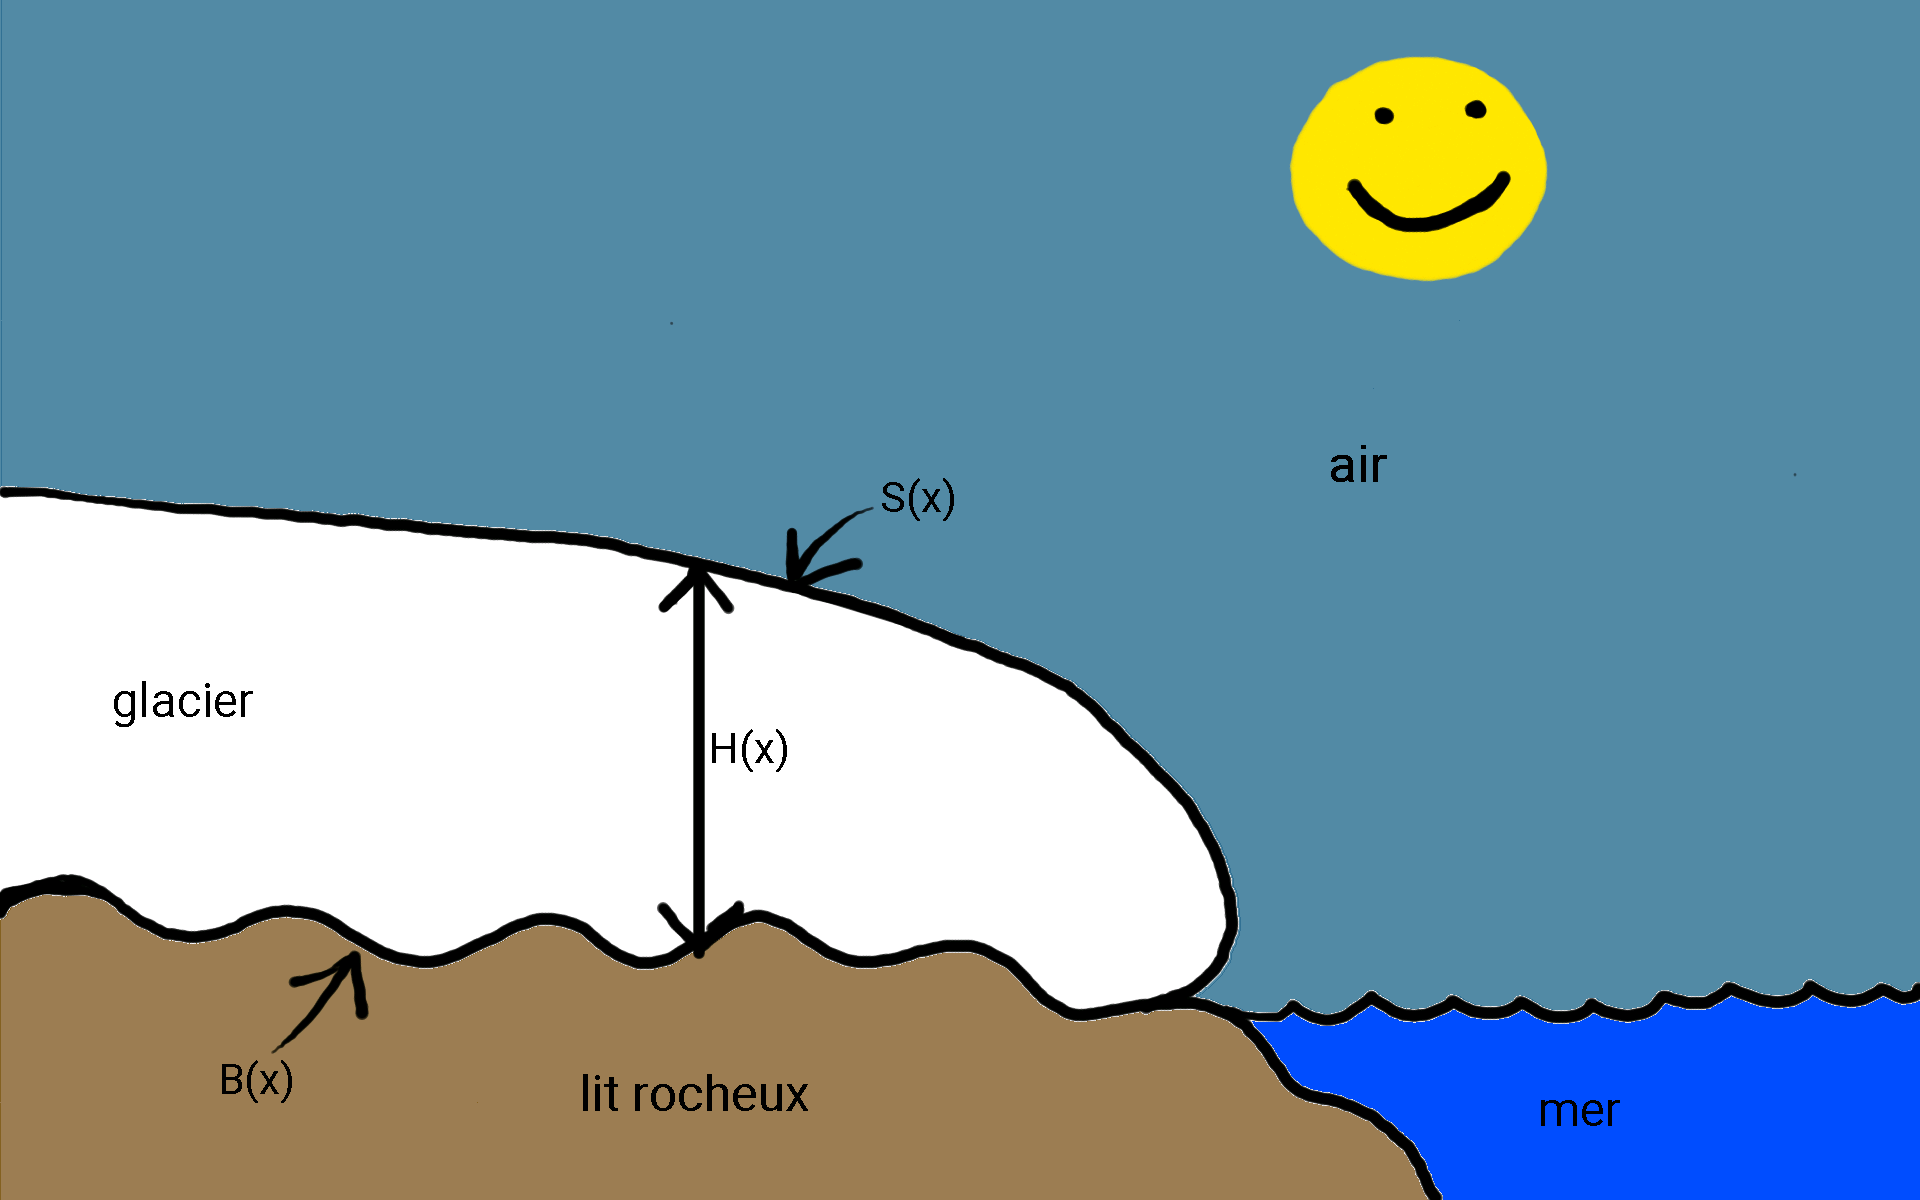
\includegraphics[width=7.5cm, keepaspectratio=true, height=7.5cm]{H.png}
\caption{Représentation de l'épaisseur de la glace H, la hauteur du lit rocheux B et la topologie de la glace S}
\label{fig01}
\end{figure}
\newline

Les données topographiques, l'élévation du substratum rocheux et l'épaisseur de la glace proviennent du jeu de données BedMachine Greenland v3. 
\\

Il faut savoir que l'écoulement d'un glacier dépend de plusieurs facteurs : la neige, glace, pluie, fonte, perte de glace, gravité. La conservation de masse M se calcule de la manière suivante :
\begin{equation}
M = accumulation + ablation
\label{5}
\end{equation}


Ainsi la conservation de masse permet d'équilibrer les 2 phénomènes à la surface en fonction de la ligne d'équilibre. L'altitude de la ligne d'équilibre (ELA) est où la zone d'accumulation, au sommet du glacier, est égale à la zone d'ablation, en bas du glacier. Nous pouvons la distinguer sur la figure \ref{fig02} : 

\begin{figure}[!htpb]
\centering
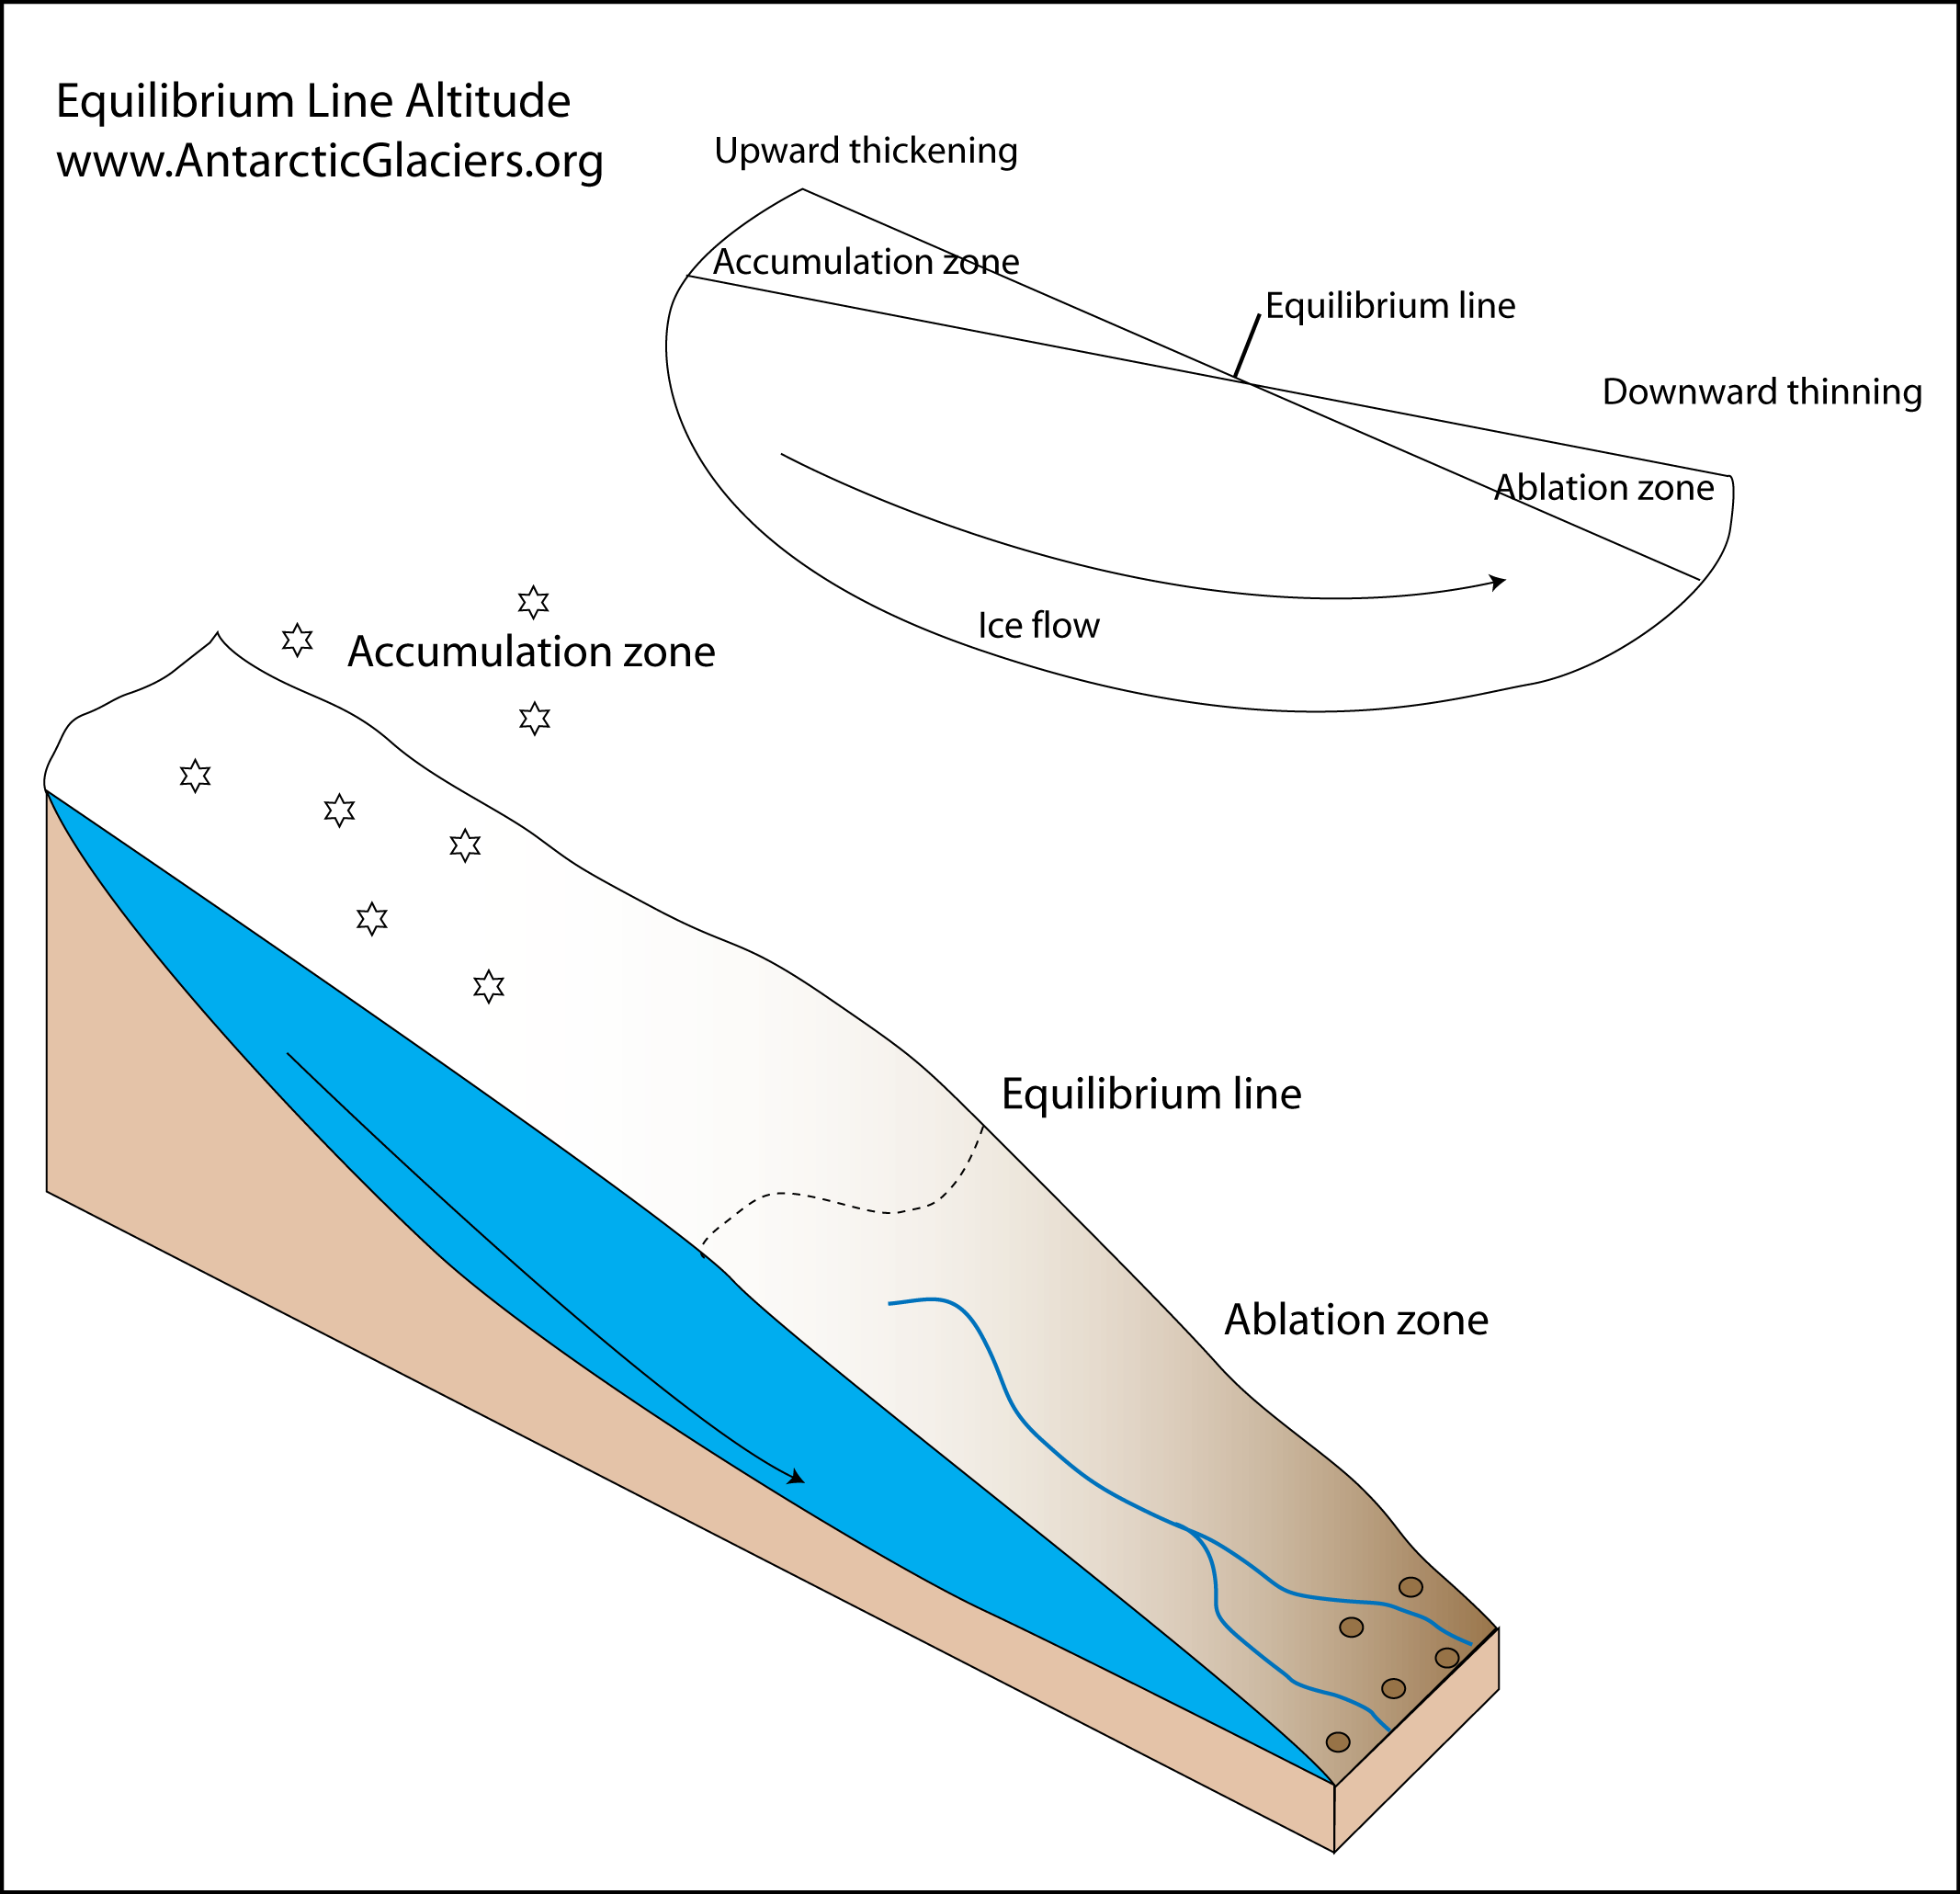
\includegraphics[width=10cm, keepaspectratio=true, height=10cm]{equilibrium_line_altitude1.png}
\caption{Représentation de la ligne d'équilibre sur un glacier, déterminée par la conservation de masse M, c'est-à-dire là où la zone d'abblation et la zone d'accumulation se rencontrent}
\label{fig02}
\end{figure}



Dans le code, la conservation de masse M est calculée à partir de $ \nabla$\textit{B} le gradient du bilan massique, \textit{zELA} l'altitude de la ligne d'équilibre (ELA) (qui dépend de la latitude) et \textit{bmax} l'accumulation maximale.
\newpage
\section{Simulations numériques}

\subsection{Les différences finies}
Pour créer nos simulations numériques, on va devoir déterminer des dérivées partielles. Mais celles-ci étant longues à calculer, nous utiliserons ici la \textbf{méthode des différences finies} afin d'approcher ces dérivées avec des calculs plus faciles et rapides.
\newline
Cependant, cette méthode étant compliquée, nous ne considèrerons que la définition suivante : On considère un intervalle et on le discrétise en plusieurs sous-intervalles.

\begin{figure}[!htpb]
\centering
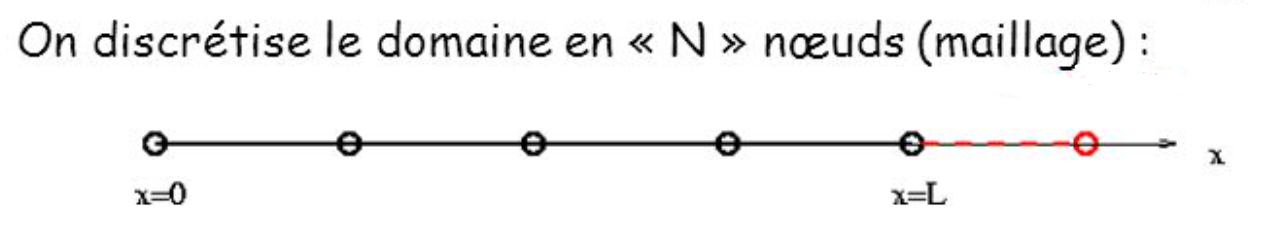
\includegraphics[width=10cm, keepaspectratio=true, height=10cm]{Differences.png}
\caption{Séparation de l'intervalle en plusieurs sous-intervalles de même taille. Afin d'obtenir une approximation de notre dérivée partielle, il suffit de prendre la valeur des deux extrêmités de chaque sous-intervalle et de faire la différence des deux.}
\label{differences}
\end{figure}

\subsection{Comprendre l'algorithme à introduire}
Nous avons commencé par étudier un dossier GITHUB public \cite{site2} qui modélisait la fonte de glacier.
\newline

 Il était composé de trois codes qui résolvent l'équation de diffusion linéaire avec différentes méthodes en 1D. 
\newline
Tout d'abord un premier code explicite qui avait pour but de nous initier à la méthode des différences finies, en calculant simplement l'équation de diffusion : 

\begin{verbatim}
 while t<ttot
        qH         .= -D*diff(H)/dx         # flux
        dHdt       .=  -diff(qH)/dx         # rate of change
        H[2:end-1] .= H[2:end-1] .+ dt*dHdt
        t += dt; it += 1
    end
\end{verbatim}
 On y applique la méthode des différences finies deux fois ce qui correspond à la dérivée seconde de H par rapport à celle de \textit{x} dans l'équation \ref{eq4}. Nous faisons cela afin de calculer dHdt que nous ajoutons à H  qui nous permet de calculer l'équation de diffusion. Ce code s'exécute au total \textit{ttot} fois.
\newpage
On a également un deuxième code qui rajoute un résiduel \textit{ResH}, une solution itérative ainsi qu'une tolérance linéaire \textit{tol}, forçant le programme à s'arrêter lorsque cette tolérance est atteinte.

\begin{verbatim}
while t<ttot
        iter = 0; err = 2*tol
        # Picard-type iteration
        while err>tol && iter<itMax
            qH         .= -D*diff(H)/dx              # flux
            ResH       .= -(H[2:end-1]-Hold[2:end-1])/dt -diff(qH)/dx
            dHdtau     .= ResH                       # rate of change
            H[2:end-1] .= H[2:end-1] + dtau*dHdtau   
            iter += 1; err = norm(ResH)/length(ResH)
        end
        ittot += iter; it += 1; t += dt
        Hold .= H
    end
\end{verbatim}
Ce \textit{err} se calcule à chaque itération gràce au résiduel \textit{ResH}. Ce résiduel est l'erreur générée par les simplifications mathématiques que l'on a créé avec la méthode des différences finies (celui-ci aurait été égal à 0 si nous avions calculé exactement nos dérivées partielles). L'erreur est déterminée avec la norme et la longueur de \textit{ResH}. Une fois que \textit{err} est inférieur à notre tolérance, nous sortons de la boucle et donc du code.
\newline
\newline
 Puis, un troisième code semblable au code implicite mais qui introduit en plus une variable \textit{damp} itérative qui permet au programme de converger plus rapidement.
\begin{verbatim}
while t<ttot
        iter = 0; err = 2*tol
        # Pseudo-transient iteration
        while err>tol && iter<itMax
            qH         .= -D*diff(H)/dx              # flux
            ResH       .= -(H[2:end-1]-Hold[2:end-1])/dt -diff(qH)/dx
            dHdtau     .= ResH + damp*dHdtau         # damped rate of change
            H[2:end-1] .= H[2:end-1] + dtau*dHdtau   
            iter += 1; err = norm(ResH)/length(ResH)
        end
        ittot += iter; it += 1; t += dt
        Hold .= H
    end
\end{verbatim}
Ce \textit{damp} est une valeur déterminée par l'utilisateur mais doit être compris entre 0 et 1. Plus ce damp est bas, plus le nombre d'itérations sera grand. Cependant, il ne faut pas prendre un damp trop grand car avec trop peu d'itérations, on risque de ne pas avoir un modèle satisfaisant (car il serait trop imprécis).
\newpage
Ces trois codes sont linéaires, car le coefficient de diffusion D est considéré comme une constante. De plus, ils considéraient le glacier comme étant une courbe parfaitement gaussienne pour ne pas avoir à extraire des données d'un autre fichier pour modéliser ce glacier.
\newline
\newline
On avait enfin un quatrième code qui résolvait le problème de l'écoulement des glaciers en 2D à l'aide du SIA. Il inclut des itérations non linéaires, c'est-à-dire que ce coefficient de diffusion D variait à chaque point et à chaque itération de la boucle, ainsi que les conditions initiales provenant des données. 
\newline
Notre but était donc de mieux comprendre le fonctionnement de ce code en 2D pour écrire à notre tour un code 1D non linéaire qui résout le problème de SIA.
\newpage
\subsection{Code 1D non linéaire proposé}
En s'inspirant de ces codes, nous avons créé notre propre code non linéaire en 1D, qui respecte l'équation~\eqref{eq4}. L'idée était de reprendre un code similaire au code non linéaire 2D et de ne conserver qu'une seule dimension, c'est-à-dire toutes les variables dépendantes de x. Les composantes dépendantes de y n'ont donc pas été prise en compte. La boucle principale s'effectue de la manière suivante :
\newline
\begin{verbatim}
while err>tolnl && iter<itMax # On sort lorsque l'erreur est en 
dessous de la tolérance 	(ou trop d'itérations)
        Err         .= H                                               
        M           .= min.(grad_b.*(S .- z_ELA), b_max)            
        dSdx        .= diff(S)/dx 
        D           .= a*av(H).^(npow+2) .*dSdx.^(npow-1)              
        qH          .= .-av(D).*diff(S[1:end-1])/dx                     
        ResH        .= .-(diff(qH)/dx .+ inn(M[1:end-1])) 
        dtau        .= dtausc*min.(10.0, cfl./(epsi .+ av(D[2:end])))
        dHdt        .= ResH + damp.*dHdt                                
        H[2:end-2]  .= max.(0.0,H[2:end-2] .+ dtau.*dHdt)               
        H[Mask.==0] .= 0.0
        S           .= B .+ H                                       
\end{verbatim}
Nous avons recréé l'équation~\eqref{eq4} en calculant les dérivées partielles selon ${x}$ avec la méthode des différences finies.
La conservation de masse M est calculé grâce à plusieurs variables qu'on prend dans les données et qu'on réévalue grâce à une fonction intermédiaire. Elle nous permet de recalculer l'accumulation de neige à chaque itération, avec une augmentation minimum de \textit{b\_max} (qu'on a considéré à 0.15m par an). La fonction utilisée a été retrouvé dans le GitHUB proposée et est la suivante :
\begin{verbatim}
function mass_balance_constants(xc, yc)
 # Permet de récupérer toutes les valeurs nécessaires pour l'ablation
    b_max    = 0.15            # max. Mass balance rate
    lat_min, lat_max = 60, 80
    Xc, Yc   = [Float32(x) for x=xc,y=yc], [Float32(y) for x=xc,y=yc]
    Yc2      = Yc .- minimum(Yc); Yc2 .= Yc2/maximum(Yc2)
    grad_b   = (1.3517 .- 0.014158.*(lat_min.+Yc2*(lat_max-lat_min)))./100.0.*0.91 
    z_ELA    = 1300.0 .- Yc2*300.0                              
    return grad_b, z_ELA, b_max
end                                   
\end{verbatim}
\newpage
Puis à partir de là, nous avons fait en sorte de n'obtenir qu'un tableau en 1D afin qu'on puisse l'utiliser dans notre code. Puis nous calculons un premier dSdx à l'aide des différences finies, qui nous servira ensuite pour calculer le coefficient de diffusion D qu'on a introduit à l'équation ~\eqref{eq5}. Ensuite on reproduit l'équation ~\eqref{eq4} en deux lignes, en effectuant deux fois les différences finies. On calcule le flux qH puis le résidu \textit{ResH} en introduisant le M précédant. Une fois que cela est fait, on calcule \textit{dHdt} en introduisant le damp itérative pour converger plus rapidement vers une solution. Une fois que cela est fait, nous réattribuons un \textbf{Mask} afin que chaque point considéré soit au minimum au niveau de la mer, et non en dessous, puis nous remettons à jour la surface S. On introduit aussi une variable \textit{cfl} qui est un coefficient suffisant pour assurer que notre modèle converge vers une solution cohérente.
\newline
\newline
Nous avons introduit plusieurs tableaux : le coefficient de diffusion D, le flux \textit{qH}, le résidu de l'équation ResH ainsi que les surfaces B, H et S, dont la taille varie en fonction des calculs qu'on leur applique. Par exemple, les méthodes des différences finies sur un tableau de taille \textit{nx} renvoie un autre tableau de taille \textit{nx-1} (car on applique \textit{nx-1} opérations sur \textit{nx} valeurs). Mais d'autres calculs directement fournis avec Julia peuvent renvoyer des tableaux de taille différente à celle d'origine, comme par exemple \textbf{av} (qui fait la moyenne des deux extrêmités pour chaque sous-intervalles) ou bien \textbf{inn} (qui renvoie le même tableau sans la première et la dernière valeur).
\newline
\newline
Ce code remet à jour toutes les valeurs jusqu'à ce que l'erreur déterminée descende en dessous d'une tolérance prédéfinie. On introduit également un pas d'itération maximal pour éviter que le programme ne s'arrête jamais.
\newline
\newline
A chaque tour de boucle, nous réinitialisons le coefficient D, la conservation de masse M et la dérivée itérative \textit{dtau}. Puis nous calculons les dérivées partielles \textit{dSdx}, \textit{qH} et \textit{ResH} en effectuant les différences finies. Toutes ces valeurs nous permettent de mettre à jour la dérivée de temps \textit{dHdt} ainsi que l'épaisseur de la glace H et enfin la surface S. Nous appliquons également un masque afin de ne pas atteindre le niveau de la mer et nous gardons en mémoire l'épaisseur H afin d'en déterminer l'erreur.
\newpage
Afin de sortir de cette boucle, nous avons introduit une \textbf{solution itérative}, semblable au code implicite décrit précédemment. Nous initialisons une variable \textit{err} et nous restons dans la boucle tant que cette erreur est supérieure à la tolérance non linéaire définie (car lorsque celle-ci sera atteinte, les variations qui suivent n'auront plus d'effet sur notre modèle). Nous avons décidé de recalculer cette erreur tous les \textit{nout} fois, qu'on a initialisé à \textbf{cinquante}, afin de ne pas faire trop de calculs. Au bout de cinquante itérations, nous actualisons la valeur de la variable \textit{err} avec le code suivant :
\begin{verbatim}
if mod(iter, nout)==0 
            Err .= Err .- H
            err = norm(Err)/length(Err) 
	    if isnan(err)
            	error("""NaNs encountered.  Try a combination of:
            decreasing `damp` and/or `dtausc`, more smoothing steps""")
            end
end
\end{verbatim}
Dans cette condition, on recalcule notre \textit{Err} en la comparant avec la hauteur de glace H actuelle. Puis on prend sa norme et on la divise par sa longueur pour obtenir notre \textit{err}. 
La boucle s'arrête lorsque l'erreur est plus petite que la tolérance imposée.
\newline
On a également une condition qui vérifie que \textit{err} est définie, c'est-à-dire qu'on vérifie que cette erreur ne tend pas vers l'infini. Cela peut arriver lorsque la longueur de \textit{Err} est nulle ou bien lorsque sa norme tend vers l'infini (ce qui peut arriver lorsqu'une des valeurs dans la boucle est mal définie). Si cela arrive, on sort du code en envoyant une erreur, signalant les étapes à effectuer pour eventuellement régler le problème.
\newline\newline
Maintenant que l'on a un modèle résolvant l'équation non linéaire H en 1D, il nous faut à présent vérifier que ce modèle est juste. Pour cela, nous avons extrait des données du Groenland datant de 2020.
\newpage

%\vspace*{\fill}
\section{Résultats}

\subsection{Extraction les données}

Pour s'assurer que le code compilait, nous avons simplifié certaines variables du problème. La conservation de masse était constante et les surfaces H, B et S  étaient modélisées par des fonctions mathématiques. Une fois cela fait, nous avons extrait des valeurs d'un autre fichier contenant toutes les valeurs du Groenland \textbf{BedMachineGreenland\_96\_176.jld}.
\begin{figure}[!htpb]
\centering
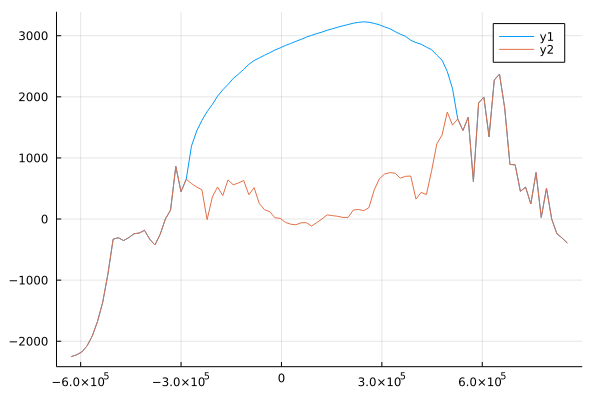
\includegraphics[width=10cm, keepaspectratio=true, height=10cm]{Groenland.png}
\caption{Topologie du Groenland d'après les données récupérées. La courbe \textit{y2} représente la hauteur du lit rocheux B et \textit{y1} la topologie de la glace S. }
\end{figure}
%\vspace*{\fill}

\
Pour l’extraction des données nécessaires, il a fallu donc charger le fichier \textbf{BedMachineGreenland\_96\_176.jld}.
Le fichier chargé est stocké dans une variable que l’on nommera \textit{var}, qui est un objet donc il va falloir extraire la valeur pour chaque clé : 

\begin{verbatim}
# Initial condition
# On charge notre fichier GeoData...
# Puis on extrait les valeurs dans les variables...
# On extrait toutes les valeurs nécessaires depuis le fichier helpers.jl...
var = load("BedMachineGreenland_96_176.jld") # ultra low res data 
Zbed = var["Zbed"]
xc = var["xc"]
yc = var["yc]
Hice = var["Hice"]
Mask1 = var["Mask"]
\end{verbatim}
\
\newpage
On obtient un objet \textit{Zbed} et \textit{Hice} qui sont plus exactement de type GeoData. Après une recherche dans la documentation de GeoData Julia, nous n’avons pas réussi à trouver comment extraire le tableau (ou la matrice) contenu dans ces objets.

Après quelques recherches sur des forums (notamment stackoverflow), puis quelques \textit{print()} dans la console, nous en avons déduit qu’il fallait faire Objet.\_clé\_, ce qui est d’ailleurs une pratique assez courante que ce soit en Python ou même en Javascript par exemple.

Ainsi on peut récupérer les informations concernant le niveau de la terre et l’épaisseur de la glace. Pour notre étude nous avons décidé de récupérer les valeurs à partir de la 80ème colonne de la matrice :

\begin{verbatim}
B1 = ZBed.data # Niveau de la terre
H1 = Hice.data # Epaisseur de la glace

# On ne récupère qu'une colonne qu'on étudiera ensuite 
# On choisit arbitrairement la colonne 80
B = B1[: , 80]
H = H1[: , 80]
\end{verbatim}
\
Une fois nos données extraites, il était nécéssaire de faire apparaître notre masque pour le niveau de la mer, que l’on a extrait dans la variable \textit{Mask1}, puis de la même manière que les valeurs \textit{Zbed} et \textit{Hice}, on récupère les données à l’aide de la clé data :
\begin{verbatim}
Mask1 = var["Mask"]
display(Mask1.data)
# Booléen qui nous permettra d'appliquer le masque pour le niveau de la mer
Mask = Mask1.data[: , 80]
\end{verbatim}
\
Nos données extraites, on peut désormais passer au traitement et à l’utilisation de notre programme.

\newpage
\subsection{Afficher un premier graphique}
\vspace*{\fill}
Nous avons ensuite réajusté l'ablation M ainsi que les coefficients itératifs damp afin d'avoir une vitesse de convergence adaptée au problème.
Nous affichons donc le résultat obtenu à l'aide d'un plot.
\begin{figure}[!htpb]
\centering
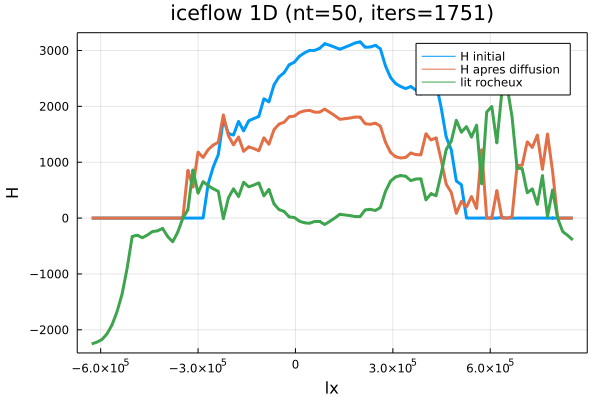
\includegraphics[width=10cm, keepaspectratio=true, height=10cm]{Iceflow1D.png}
\caption{Evolution du niveau de glace en fonction du temps. La courbe bleue représente la hauteur H au début, la courbe orange donne la hauteur H une fois la simulation terminée et la courbe verte montre le lit rocheux B.}
\end{figure}
\vspace*{\fill}

\newpage
\subsection{Chercher une situation proche du code 2D}

Il nous faut à présent déterminer la ligne où les variations verticales soient les plus faibles, afin d'avoir le modèle le plus proche possible de la réalité adapté à notre code.
\newline
Pour cela, nous avons cherché dans les données que nous avions sur le Groenland la ligne "horizontale" qui nous permettait d'avoir des résultats suffisamment justes pour pouvoir appliquer notre code. Plus précisément, il fallait que la ligne choisie soit une ligne qui permette de négliger les vitesses verticales.
Pour choisir judicieusement cette ligne, nous avons comparé les différentes données de vitesses verticales \textit{Vy} que nous avions à notre disposition en faisant une somme entre deux lignes consécutives, voici le code qui nous a permis de trouver  la ligne correspondante: 
\begin{verbatim}
V = sqrt.(Vy.^2)
s=zeros(95)
for i = 1:95
    t=V[i,:]
    s[i]=sum(t)
end

for i = 2:94
    s1[i-1] = s[i-1] + s[i+1]
end
display(plot(1:95, s))
display(plot(1:94, s1))
\end{verbatim}

\newpage

\vspace*{\fill}
A l'aide de ce programme, nous pouvons obtenir une courbe donnant les vitesses verticales sur chaque ligne :
\begin{figure}[!htpb]
\centering
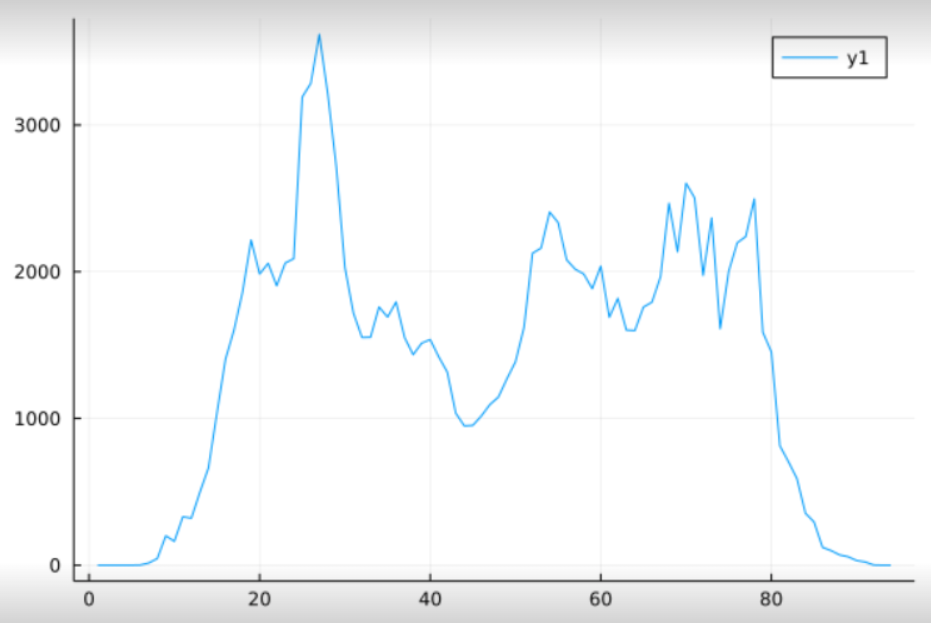
\includegraphics[width=10cm, keepaspectratio=true, height=10cm]{Vitesses.png}
\caption{Graphe représentant la somme des variations verticales par rapport aux lignes du Groenland. On ne considère pas les bordures du Groenland car on veut prendre la ligne qui correspond au rapport entre la vitesse horizontale et verticale la plus élevée, ceci est situé au centre du Groenland }
\end{figure}
\newline
 En regardant au centre, nous observons que les vitesses verticales sont les plus faibles vers la ligne 43. Nous avons alors choisi cette ligne pour que notre modèle soit le plus cohérent avec notre modèle 2D. 
\vspace*{\fill}

\newpage

En exécutant le code avec cette ligne, nous avons alors le résultat suivant: 
\begin{figure}[!htpb]
\centering
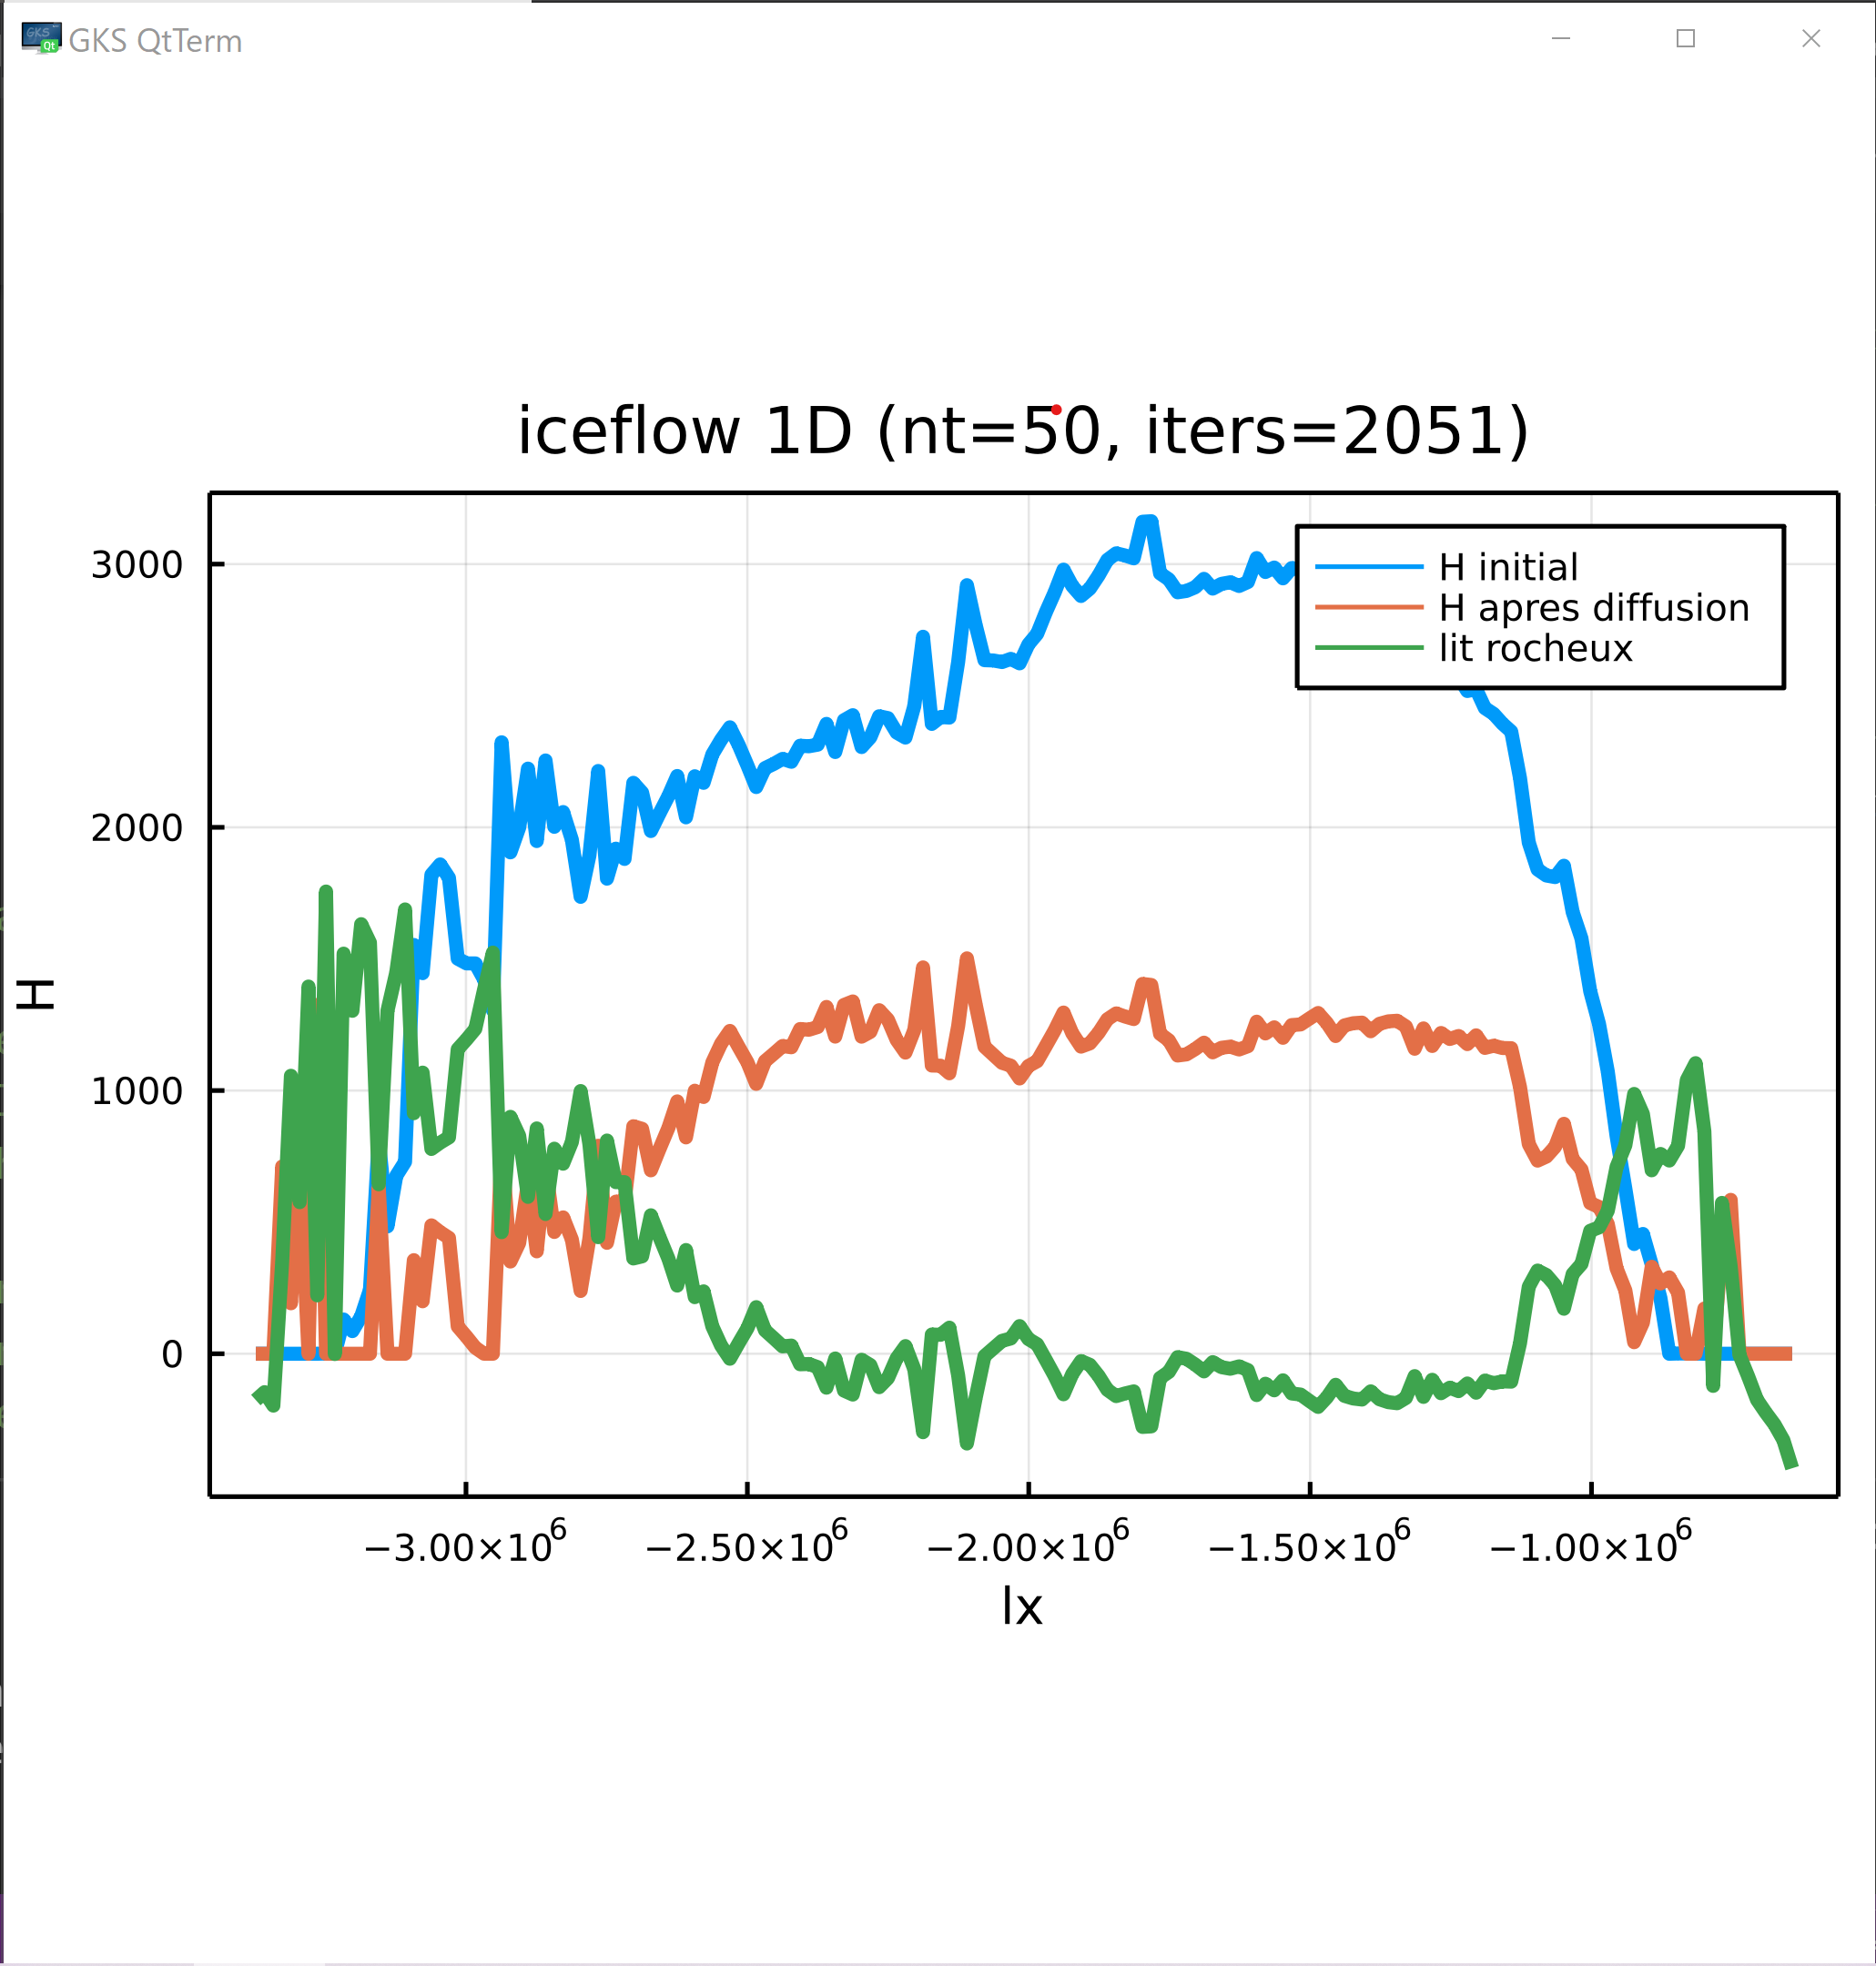
\includegraphics[width=10cm, keepaspectratio=true, height=10cm]{ligne43.png}
\caption{Topologie du Groenland en appliquant la ligne 43. La courbe bleue  représente la hauteur H au début, la courbe orange donne la hauteur H une fois la simulation appliquée pour la ligne 43 et la courbe verte montre le lit rocheux B. }
\label{ligne43}
\end{figure}

\subsection{Interpréter notre simulation}

En observant notre schéma, nous pouvons à présent simuler l'évolution de la glace du Groenland et créer notre propre scénario. En observant nos valeurs, nous pouvons observer une fonte de glace allant de 0 à 1500m de variation. 
\begin{verbatim}
    fonte = zeros(nx)
    fonte = H0 .- H
    moy0 = sum(H0)
    moy = sum(fonte)
    @printf(" Hauteur de base moyenne est : %d , 
Fonte moyenne est : %f ",moy0/length(H0) ,moy/length(fonte))
\end{verbatim}
\newpage
Avec un simple calcul de moyenne, nous obtenons une variation moyenne de 1091m. Notre hauteur de base moyenne étant de 1907, cela nous donne une variation de 57\% de la hauteur. A chaque itération, nous réattribuons des valeurs à tous les tableaux en fonction de a, qui est la viscosité de la glace \textbf{calculée avec un pas de temps annuel}. Nous en déduisons qu'une itération correspond à une année et donc que ce scénario sera atteinte au bout de 2051 ans. 
\newline
Nous avons trouvé un article de \textbf{ Geophysical Research Letters} \cite{charbit2008amount} spéculant la fonte de glace au Groenland en fonction de la hausse de CO2, car celui-ci est directement relié avec la hausse de température. Il effectue plusieurs simulations, en fonction de la variation de température considérée (variant entre 1.1°C et 6.4°C) : 
\begin{figure}[!htpb]
\centering
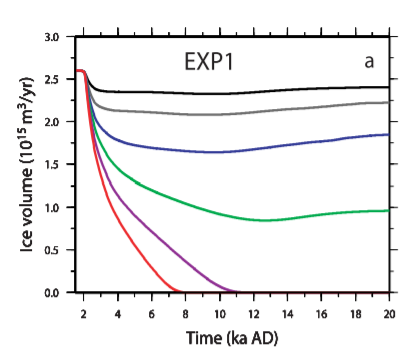
\includegraphics[width=10cm, keepaspectratio=true, height=10cm]{Variation.png}
\caption{Schéma indiquant le volume de glace du Groenload à partir de l'an 2000. Grâce à cette simulation, nous pouvons en déduire que le Groenload perdrait entre 10\% et 63\% de son volume, ce que l'on retrouve bien avec notre simulation (Notre simulation est proche de la courbe verte de ce schéma) }
\end{figure}
\newpage
\subsection{Modifier nos valeurs itératives}

Etant donné que nous avons introduit des valeurs itératives comme damp, nous avons voulu savoir ce qu'on allait obtenir lorsqu'on faisait varier cette valeur. Nous avons donc pris deux valeurs extrèmes 0.1 et 1 et nous avons tenté d'afficher le modèle obtenu :
\begin{figure}[!htpb]
\centering
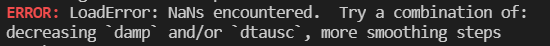
\includegraphics[width=10cm, keepaspectratio=true, height=10cm]{Damp01.png}
\caption{Résultat du plot de notre code lorsque damp est à 0.1. Cela montre bien qu'avec trop peu d'itérations, notre modèle est incapable d'afficher une modélisation cohérente.}
\end{figure}

\begin{figure}[!htpb]
\centering
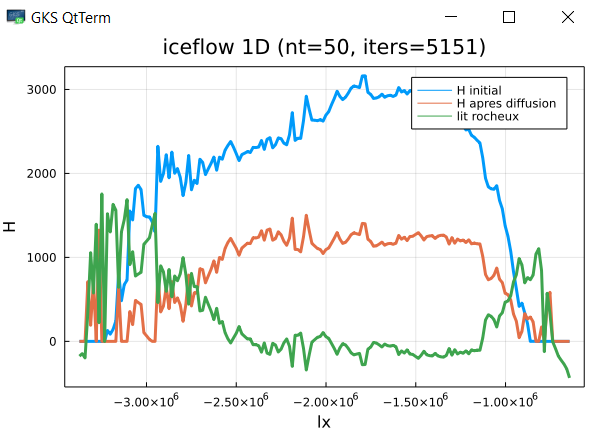
\includegraphics[width=10cm, keepaspectratio=true, height=10cm]{Damp1.png}
\caption{Résultat du plot de notre code lorsque damp est à 1. On remarque que le résultat obtenu est semblable à celui présenté à la figure \ref{ligne43}, mais on a fait un nombre d'itérations bien plus important pour parvenir à ce résultat. Cela montre bien l'intérêt d'avoir un damp permettant de réduire le temps de modélisation.}
\end{figure}
\newpage
%-----------------------------------------------------------
\bibliography{bibliographie.bib}
\bibliographystyle{unsrt}
\end{document}

